% Figure Q1, generated by experiments/q1_sum_vs_sq.py.
% \input this from a results section; do not include the PNG directly.
\begin{figure}[t]
  \centering
  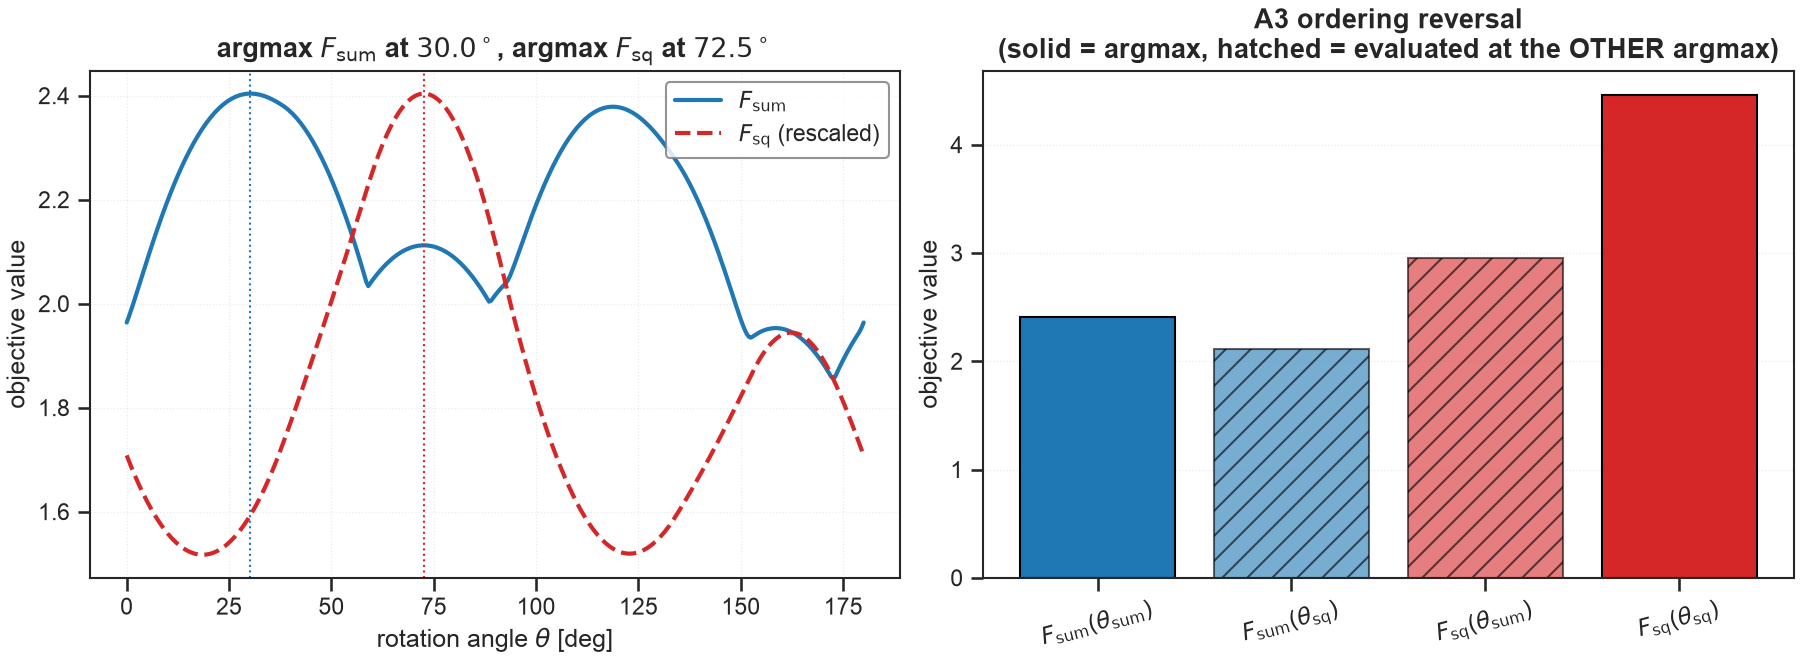
\includegraphics[width=\linewidth]{../shared/figures/generated/q1_sum_vs_sq.png}
  \caption{\textbf{Q1, A-SUM and A-SQ disagree at $m\!\ge\!2$.} Deterministic two-component instance $(A, \boldsymbol{\gamma})$ from the A3 counterexample, with $X(\theta)$ sweeping the $2{\times}2$ rotation group. \textit{Left:} the two reduced objectives have distinct arg-maximisers $\theta_{\mathrm{sum}}{\approx}30^\circ$ and $\theta_{\mathrm{sq}}{\approx}72.5^\circ$. \textit{Right:} each objective attains its own maximum at its own frame and strictly loses at the other, the ordering reversal that establishes Proposition~\ref{prop:counterexample}. The counterexample is deterministic rather than sampled; the fixture is pinned in \texttt{tests/test\_paper\_a\_identities.py::test\_a3\_sum\_vs\_squared\_aggregation\_rank\_two\_candidates\_differently}.}
  \label{fig:q1-sum-vs-sq}
\end{figure}
